%!TEX encoding = UTF-8 Unicode
% !TeX spellcheck = en_GB
%%%%%%%%%%%%%%%%%%%%%%%%%%%%%%%%%%%%%%
\chapter{Experimental measurements of the Higgs boson }\label{chap:HiggsConstr}
%%%%%%%%%%%%%%%%%%%%%%%%%%%%%%%%%%%%%%
The observation of the Higgs boson, followed by the extensive measurement of its properties and couplings, has been on the top of the LHC programme priorities~\cite{ellis2000physics}. When this thesis was written, the particle physics community was celebrating a decade since the Higgs boson's discovery. Looking back ten years from now, when I have witnessed the discovery of the Higgs boson via a news press conference in the Summer of 2012 and decided to be a part of this enormous step that humanity has taken.
I feel astonished by the progress made in understanding the last piece of the SM to be unravelled!  \\ In this chapter, I will start with an overview of the extraordinary LHC and its experiments~in~\autoref{sec:theLHC}. Then, I will provide a state-of-the-art status review of the experimental measurements of the Higgs boson properties in~\autoref{sec:Higgsprop} and its cross-sections and couplings in~\autoref{sec:Higgscoupl}. An the end, I will discuss the challenges and outlook for the future runs of the LHC~\autoref{sec:Higgscouplchallenge}. The rest of the thesis will address a small part of these challenges.
%%%%%
\section{Overview of the Large Hadron Collider \label{sec:theLHC}}
%%%%%aa
\par The Large Hadron Collider~(LHC) is the largest particle accelerator in the CERN accelerators complex, with a circumference of about 26 \si{\kilo\metre} and over 9590 superconducting magnets that are cooled to 1.9 \si{\kelvin}. It was built as an upgrade the Large electron-positron collider~(LEP), which ended its operation in the year 2000. The LHC contains four main experiments situated at the four beam crossing points: ATLAS, CMS, LHCb and ALICE. There are also smaller experiments such as LHCf, MilliQan,TOTEM and others. For more details about the LHC cf.~\cite{cernfacts,welt-machine}, or the LHC technical design report~\cite{Bruning:2004ej} for an in-depth review.\\   The LHC started operation in September 2008, with low energy proton beams, then gradually increased to an energy of 3.5 \TeV\ per proton to reach a centre of mass energy of~$\sqrt{s}$ of 7 \TeV. The data-taking period started in 2011. By 2012, its energy had increased to $\sqrt{s}= 8\ \TeV$ and operated at this energy for about a year and a half, followed by a stopping its operation in mid-2013, concluding what is known as \textbf{Run-I}. In 2015,  \textbf{Run-II} has started with almost double the energy $\sqrt{s}= 13\ \TeV$, and lasted for ca. 3 years. As this thesis is written, preparations are being made to get \textbf{Run-III} started and it will last until 2024. During these runs, heavier nuclei such as $\prescript{207}{}{\mathbf{Pb}}$ and $\prescript{131}{}{\mathbf{Xe}}$ have been collided either with protons or with themselves~\cite{lhckomission}.  \\  From, 2025 and beyond, the \textbf{High-Luminosity} LHC~(HL-LHC) era will commence, see~\autoref{fig:lhcplan}.  The LHC will be shut down for extensive upgrades ~\cite{Apollinari:2015bam} to potentially increase its energy up to~$\sqrt{s}= 14\ \TeV$ and increase its collision rate; hence the name \emph{high luminosity} is given for this operation period. This leads us to an important notion in particle physics phenomenology ~\emph{integrated luminosity}.\\
\par The performance of a particle collider depends on many factors, but for phenomenological studies, like this thesis, the most important of which are the centre-of-mass energy $\sqrt{s}$ and the integrated luminosity~$\mathscr{L}$.
This is mainly because particle-collider experiments are basically ``counting experiments''. All of the discoveries or bounds on physical observables are obtained from the number of signal versus background events.  In a collider, the number of expected events~$N_{expec}$ for a given resonance $R$ and a subsequent decay final state $X$ at any collider experiments is given by
\begin{equation}
	N_{expec} = \sigma(pp\to R) \, \mathrm{BR}(R \to X)\,\mathscr{L}  \, \epsilon_{\mathrm{SEL}}.
	\label{nevents}
\end{equation}
 Where $\epsilon_{\mathrm{SEL}}$ is the selection efficiency, which depends on many factors like the detector geometry and particle identification performance etc., as well as the nature of signal at hand; it can be improved by better detected or selection cuts. The production cross-section increases typically quadratically with $\sqrt {s}$, hence comes the need for higher energies, but this can only be achieved by building new colliders from scratch. On the other hand, the integrated luminosity can be increased by running the experiment for a longer period of time without the need for a new collider. This is because the integrated luminosity is the time integral of the collider's luminosity $L(t)$ over its operation time $T$
\begin{equation}
	\mathscr{L} = \int^{T} L(t) .
\end{equation}
Therefore, we see that the integrated luminosity for the LHC experiments will increase over time as more collisions take place. ~\autoref{fig:lumi} shows the integrated luminosity for ATLAS and CMS experiments as it increases with each operation period of the LHC. 
\begin{figure}[t!]
	\begin{center}
		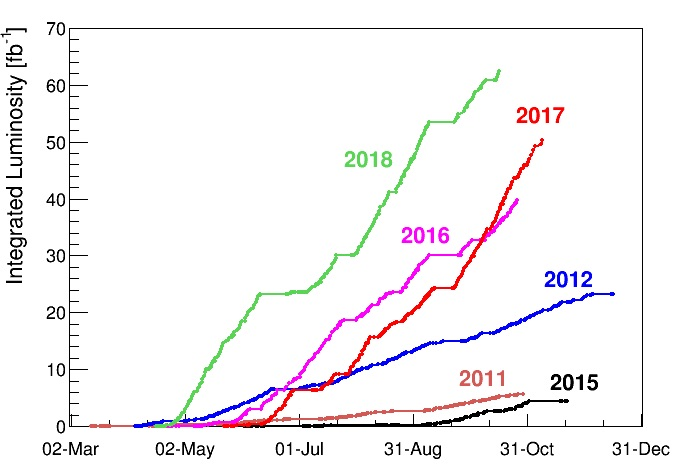
\includegraphics[width=8cm]{figures/lhc_lumi}
		\caption{The integrated luminosity of the CMS and ATLAS experiments combined over the operation period from 2011-2018, source~\cite{lhcpreformance}.  \label{fig:lumi} }
	\end{center}
\end{figure}
Protons travel in the LHC in \textbf{bunches}, when these bunches cross, the protons inside of them collide at a certain frequency $f$.  When two bunches with $N_1$ and $N_2$ protons per bunch, respectively collide, each bunch will have an effective cross-section~$4 \pi \sigma_i$ corresponding to their physical sizes $\sigma \sim \SI{16}{\micro \meter}$, the luminosity is therefore given -approximately- by 
\begin{equation}
	L = \frac{f N_1 N_2}{4 \pi  \sigma_1 \sigma_2},
\end{equation}
which is for the LHC averages to  $\sim 10^{34}$ collisions \si{\per \centi\metre\squared \per \second}~\cite{closer,lhcpreformance}.  \\ The total physics-viable $pp$-collisions  integrated luminosity for Run-I was \SI{4.57}{\infb} for \SI{7}{\tera\electronvolt} and \SI{20.3}{\infb} for \SI{8}{\tera\electronvolt} (ATLAS~\cite{atlaslumi1}) and  \SI{5.55}{\infb} at \SI{7}{\tera\electronvolt} and \SI{21.8}{\infb} at \SI{8}{\tera\electronvolt} (CMS ~\cite{cmslumi}). As for Run-II the integrated luminosity is \SI{139}{\infb} at \SI{13}{\tera\electronvolt } (ATLAS~\cite{atlaslumi2})  and \SI{137}{\infb} at \SI{13}{\tera\electronvolt } (CMS ~\cite{cmslumi}). The expected integrated luminosity by the end of Run-III is  \SI{300}{\infb}~\cite{Fartoukh:2790409} and \SI{3000}{\infb} by the end of the HL-LHC at energy of \SI{14}{\tera\electronvolt }~\cite{Apollinari:2015bam}. 
%\begin{sidewaysfigure}[ht]
\begin{figure}[htbp!]
	\centering
	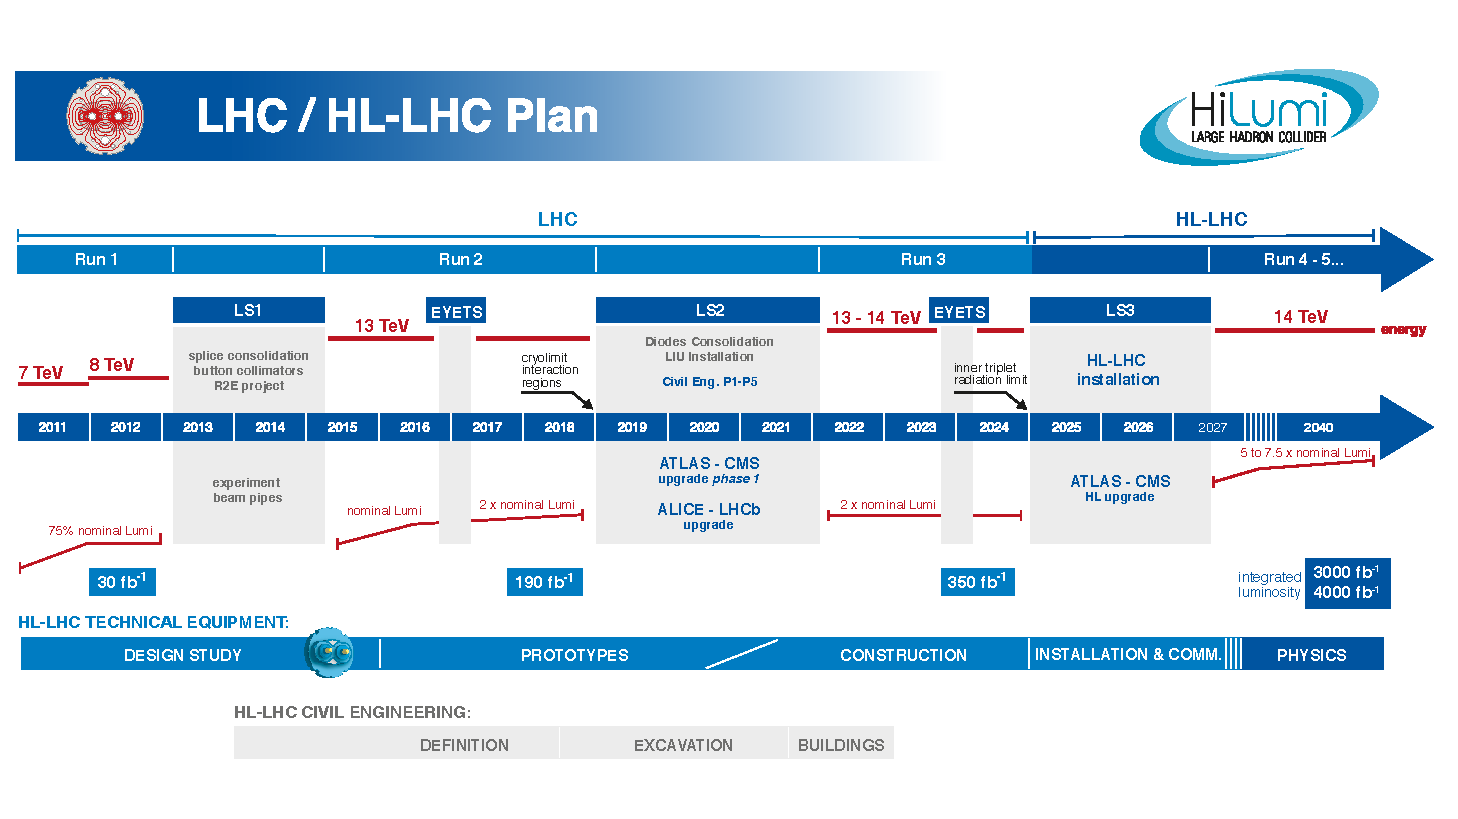
\includegraphics[width=\textwidth]{figures/HL-LHC-plan-2021-1}
	\caption{ A timeline of the LHC operation showing Run-I, Run-II and future planned runs of the LHC, including the HL-LHC, source~\cite{lhckomission}. 
	}
	\label{fig:lhcplan}
\end{figure}
%\end{sidewaysfigure}
%\FloatBarrier
\section{Higgs properties \label{sec:Higgsprop} }
\subsection{Higgs boson mass measurements}
To measure the mass of the Higgs boson with high precision, one needs to consider final states that can be reconstructed with high momentum and mass resolutions. This is typically achieved when no hadronic constituents in the decays are involved, such as  $ h \to \gamma \gamma$ and $ h \to Z Z^*\to 4 \ell$. Reconstructing the invariant mass distributions $m_{\gamma \gamma}$ and $m_{4\ell}$ one observes that the Higgs peak is narrow over a relatively smooth background, see~\autoref{fig:higgs_mass}; this is ideal for the measurement of the Higgs mass. It should be noted that the width of the resonance is due to the detector resolution and does not correspond to the actual Higgs width.\\
\begin{figure}[t!]
	\begin{center}
		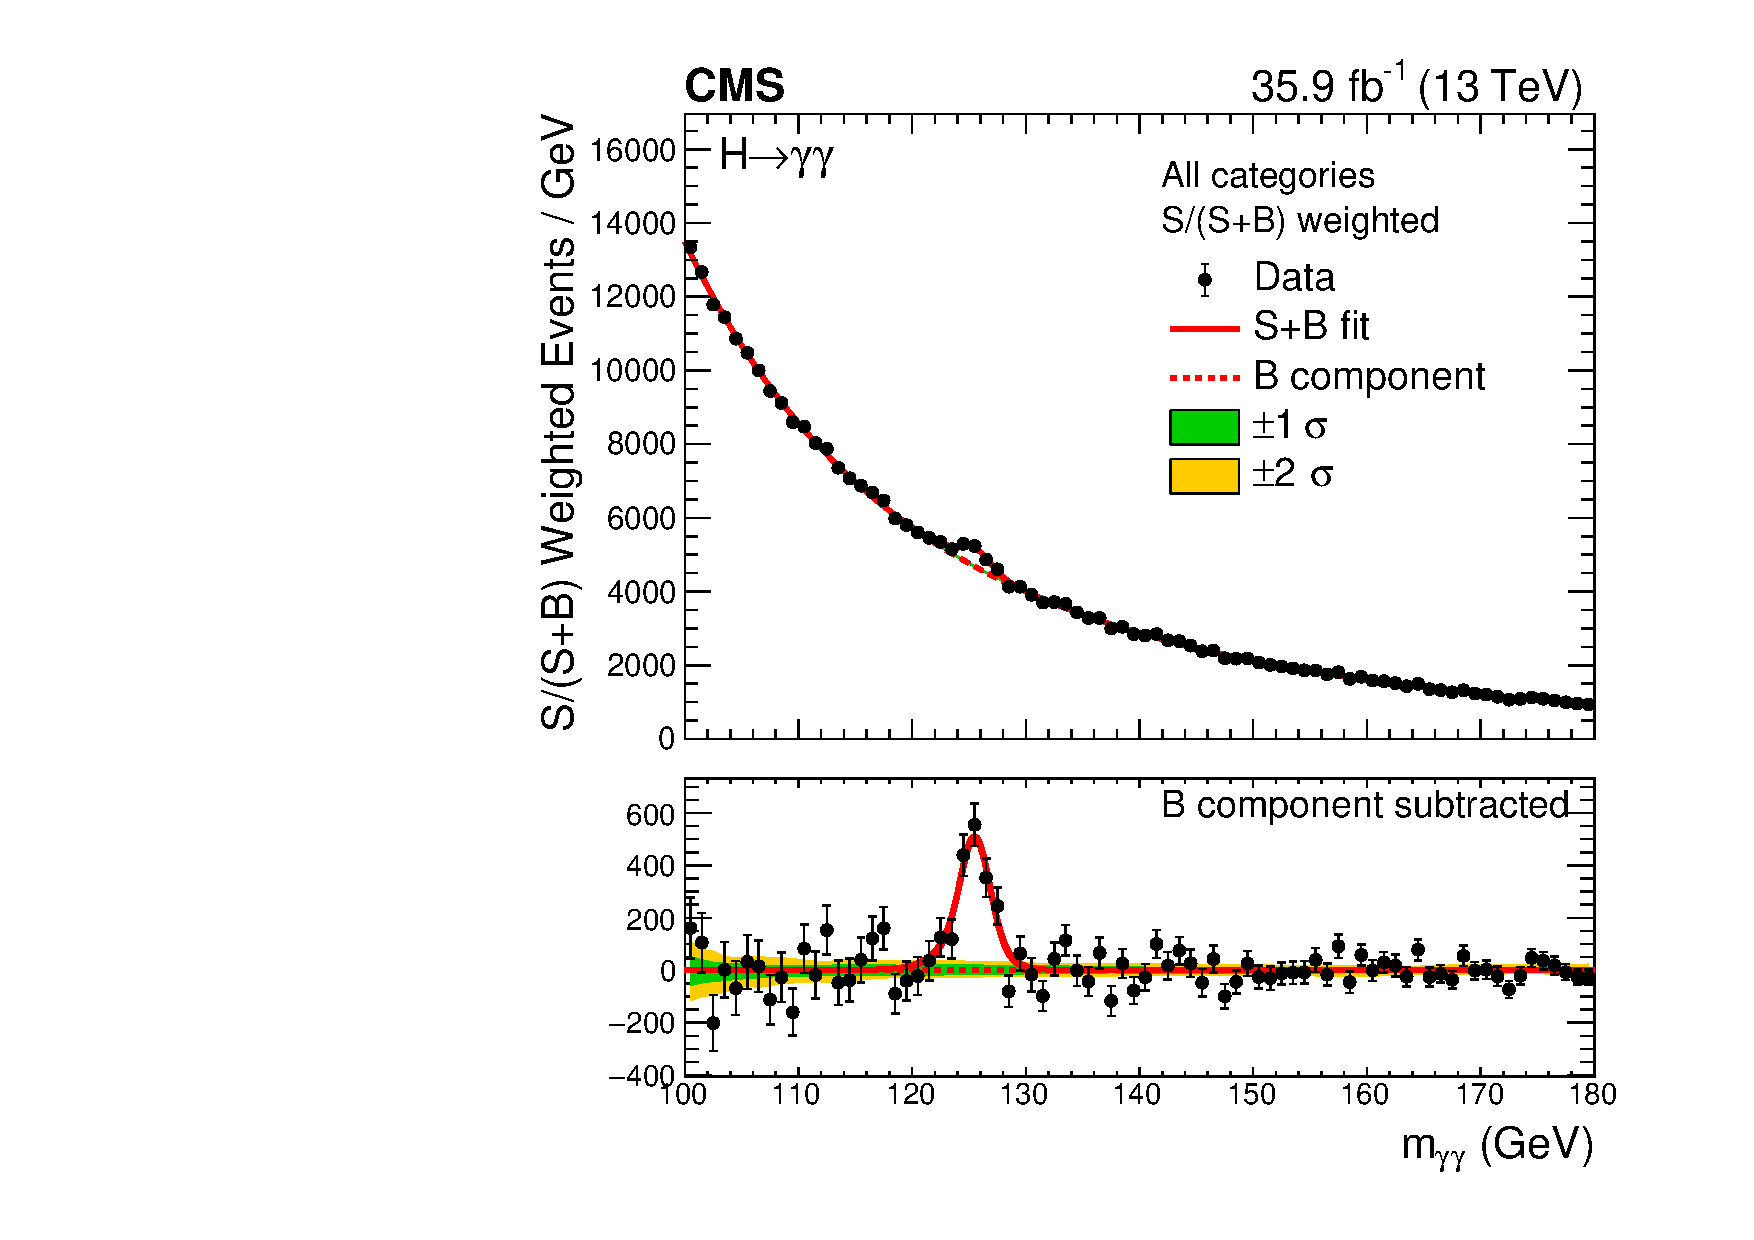
\includegraphics[width=0.45\textwidth]{figures/Higgs_results/CMS-HIG-19-004_Figure_005-b}
		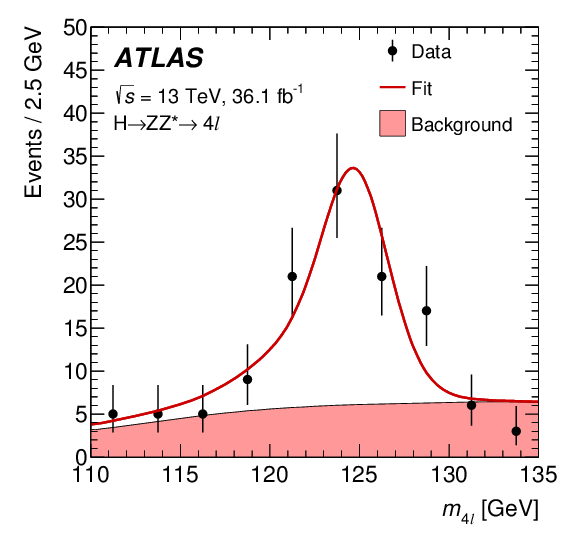
\includegraphics[width=0.45\textwidth]{figures/Higgs_results/dataAll_H4l_m4l_pdf_constrained} 
		\caption{The invariant mass distributions of diphoton~$m_{\gamma \gamma}$ (CMS~\cite{CMS:2020xrn}) and four lepton $m_{4 \ell}$ (ATLAS~\cite{ATLAS:2018tdk}) final states showing a clear peak at the Higgs mass, with smooth background. These final states are ideal for Higgs mass measurements. The figures are taken from their respective references. \label{fig:higgs_mass} }
	\end{center}
\end{figure}
There have been consistent improvements of the Higgs mass measurements since its discovery. In~\autoref{fig:meta_mass}, I have preformed a meta-analysis on ATLAS and CMS measurements of the Higgs mass in Run-I and Run-II of the LHC for both diphoton and $ZZ^*$ final states based on the data from the studies~\cite{ATLAS:2015yey,ATLAS:2018tdk,CMS:2017dib,CMS:2020xrn} using a random effects model~\cite{aronow_miller_2019}, the random effect variable is the study itself. The pooling of the studies yielded a mass measurement of $ m_h = 125.21 \pm 0.10$ that translates to a $0.11\%$ accuracy. The heterogeneity of the studies is found to be $I^2 =49\%$ ($p=0.05$). Different measurements combination techniques were used in~\cite{CMS:2020xrn} and~\cite{Zyla:2020zbs} yielded a slightly different central values but all of the results agree within the uncertainties. 
\begin{figure}[h!]
	\begin{center}
		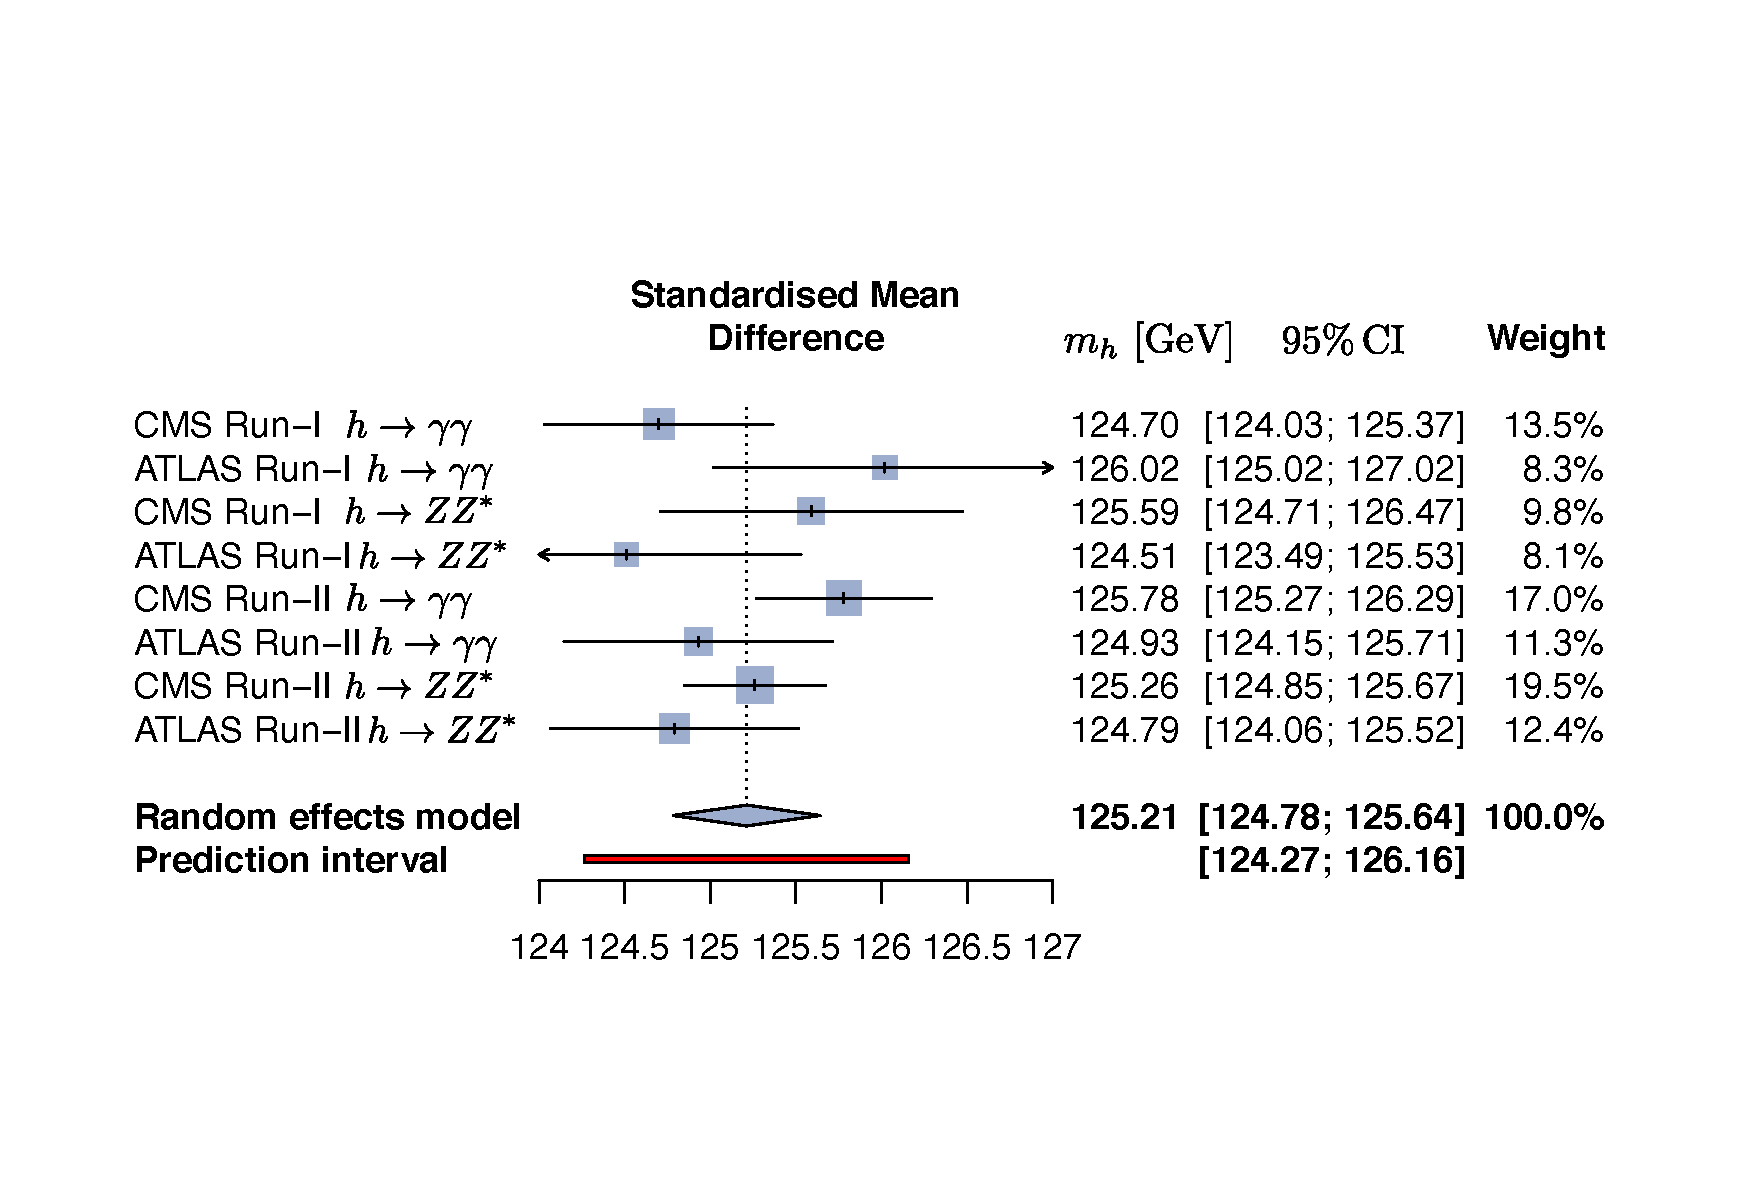
\includegraphics[width=1.\textwidth]{figures/foreest_pllot_higgs_mass}
		\caption{A meta analysis preformed to combine all the measurements of the Higgs mass from Run-I and Run-II, the combined result was obtained from pooling all of the studies using the random effects model method.\label{fig:meta_mass} }
	\end{center}
\end{figure}
\subsection{Higgs full width}
The SM values of the Higgs boson full width i~$\Gamma_h=4.1$ \GeV\, and it can be accessed in the LHC by looking at the ratio of on-shell vs off-shell Higgs production and decay to the $ZZ^{(*)}$ state, and $ZZ^{(*)}\to 4 \ell, 2 \ell 2 \nu$, namely
\begin{equation}
	\frac{\sigma(gg \to h\to Z Z^*)}{\sigma(gg \to h^*\to Z Z)} = \kappa_g^2 \kappa_Z^2 \frac{4 m_Z^2}{m_h \Gamma_h},
	\label{widthform}
\end{equation}
where the $\kappa$ here denotes the ratio between the measured or modified coupling with the Higgs and the SM prediction, i.e.
\begin{equation}
	\kappa_X := \frac{g_{XX h}}{g_{XXh}^{\SM}}.
	\label{kappa}
\end{equation}
The $\kappa$-formalism is commonly used in reporting experimental constrains/ of the Higgs couplings; it will be discussed in more detail in~\autoref{chap:HiggsEFT}. \\  Unfortunately, it is not possible to directly measure the Higgs full width at the LHC, as this requires full reconstruction of the collision event and study the recoil mass, and this is only possible at lepton colliders~\cite{DeBlas:2019qco,Banerjee:2021huv}. 
Alas, it is still possible to extract bounds on $\Gamma_h$ using ~\eqref{widthform}. ATLAS used this method to constrain the full width of the Higgs using Run-II data~\cite{ATLAS:2018jym}, while CMS has preformed the same analysis using Run-I and Run-II data combined~\cite{CMS:2019ekd}, the results are 95\% CL bounds of $\Gamma_h$
\begin{align}
	\Gamma_h &< \SI{14.4}{\giga\electronvolt} \,\,\,\, (\text{ATLAS}) & \SI{0.08}{\giga\electronvolt} <&\Gamma_h < \SI{9.16}{\giga\electronvolt}  \,\,\,\, (\text{CMS}),
\end{align}
with the combined bound approaching  $\sim 3 \Gamma_h^{\SM}$. 
\subsection{Higgs spin and parity \label{higgscp}}
According to the SM predictions, the Higgs boson in a scalar and $\mathcal{CP}$ even ($J^p= 0^+$). However, the discovery of a peak in the $m_{\gamma \gamma}$ distribution on its own would not automatically imply that the particle discovered is scalar; it could be a spin-$2$ boson or a pseudoscalar  ($J^p= 0^-$). To study the $J^p$ properties of the Higgs, one needs to examine the differential distributions of angular variables such as the rapidity~$y$ or transverse momentum~$\pt$. Both ATLAS and CMS collaborations studied the angular distributions of the Higgs decays $ h \to ZZ^*$, $h \to W W^*$ and $ h \to \gamma$, then tested the alternative hypothesis for $J^p$ against the SM~\cite{ATLAS:2015zhl, CMS:2014nkk}.  The analysis results showed that the SM ~$0^+$ hypothesis is favoured at $ >99.9\%$ CL. 
\section{Measurements of Higgs rates and couplings \label{sec:Higgscoupl} }
\subsection{Higgs cross-sections}
\par The total inclusive Higgs boson cross-section has been measured using the the final states $ h \to \gamma \gamma$ and $ h\to Z Z^* \to 4 \ell$, and their combinations.  The measurements have been done at the three energies of the LHC : 7 TeV, 8 TeV ~\cite{CMS:2015zpx} and 13 TeV~\cite{CMS:2018gwt,CMS:2021ugl,ATLAS:2019mju}. As shown in~\autoref{fig:xstothiggs}, the measured inclusive cross-section is in agreement with the SM prediction across all of the LHC operation energies.
\begin{figure}[htb!]
	\begin{center}
		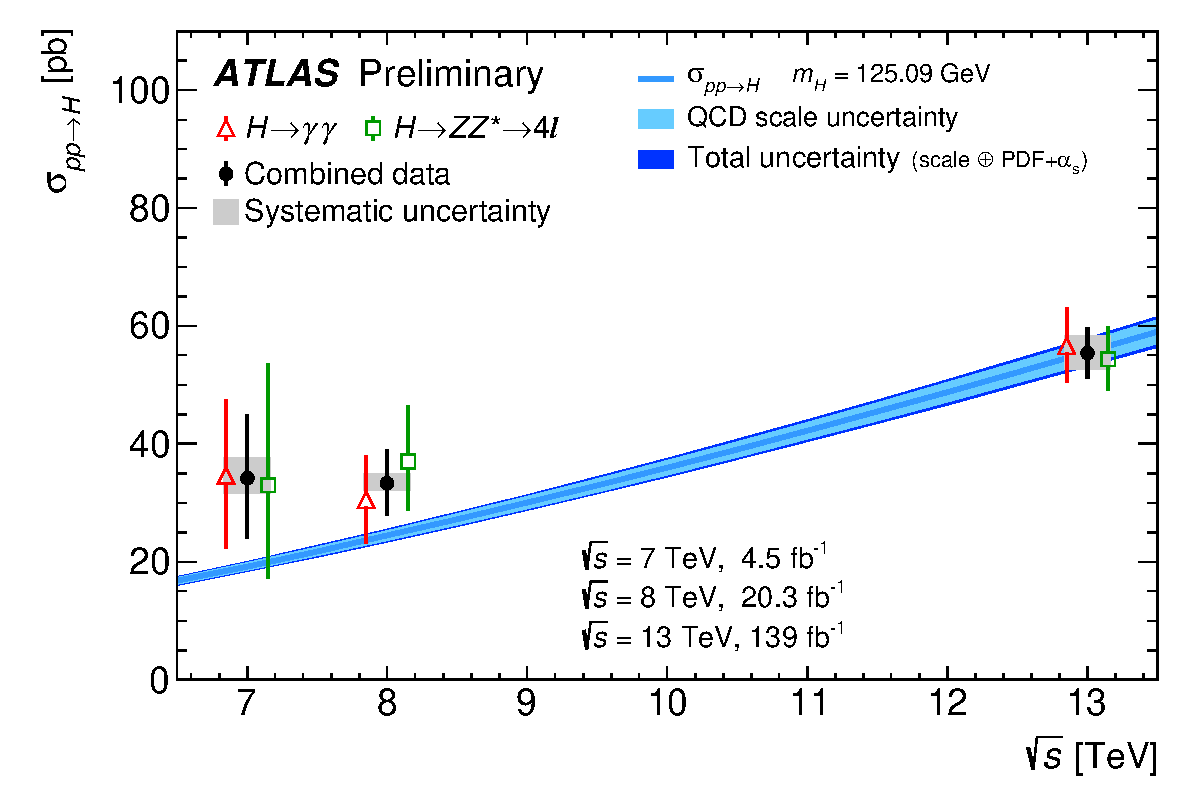
\includegraphics[height=0.35\textheight]{figures/Higgs_results/fig_01}
		\caption{The total inclusive cross-section measurements by ATLAS collaboration~\cite{ATLAS:2019mju} for $7$, $8$ and $13$ TeV using  $ h \to \gamma \gamma$ and $ h\to Z Z^* \to 4 \ell$. channels and their combination (black points) compared to the SM prediction with the  uncertainties shown as blue line with light and dark blue bands for QCD scale uncertainties and total uncertainties, respectively. This plot is taken from the quoted results.}	
		\label{fig:xstothiggs}
	\end{center}
\end{figure}
%\FloatBarrier
\par In addition to the inclusive cross-section measurements,  differential cross-sections of the Higgs has been measured for $\pt$ and  $y$ as we have seen in~\autoref{higgscp} for Higgs's $J^p$ determination. Additionally,  the differential cross-sections for other variables have been studied including $N_{jets}, \pt^{jet}, m_{jj},\delta \phi_{jj}$ and others.  The channels $ h \to ZZ^*$, $h \to W W^*$ and $ h \to \gamma$ were used for these studies. The most recent results using the full Run-II data can be found in~\cite{CMS:2018gwt,ATLAS:2019jst,ATLAS:2019mju,CMS:2019chr}.  \\
A collection of measurements of Higgs production and decay rates has been carried out by both ATLAS and CMS. These measurements are also carried out in what is known as the ``Standard Template Cross-Sections''~(STXS) framework. The STXS is fiducial cross-sections in exclusive phase-space regions or bins stratified by the Higgs boson production channels. They have the advantage of standardisation of cuts and final results such that measurements could be easily combined across analyses. More details about the STXS framework can be found in the reports of  LHC Higgs cross-sections working group~(HXSWG)~\cite{Berger:2019wnu}.  \autoref{table:resHiggsExp} presents a summary of the state-of-art measurements of the Higgs rates separated into production and decay channels using the total LHC Run-II data from ATLAS and CMS experiments. The HL-LHC projections from the CMS experiment are given as a comparison. The results in this table are written in terms of the signal strength, which is directly extracted from measuring the number of events dividing them by the SM prediction
\begin{equation}
	\mu_{\mathrm{Exp}} := \frac{ \sigma \cdot \mathrm{BR}}{ \sigma^{\SM} \cdot \mathrm{BR}^{\SM}}.
\end{equation}
\newpage
\begingroup
\thispagestyle{plain}
\begin{table}[htb!]
\centering
\vspace{-1 cm}
 \footnotesize{ 
	{\renewcommand{\arraystretch}{0.75 }%
\begin{tabular}{clccc}
\toprule
\toprule
\multirow{5}{*}{ {\normalsize Production}}  &\multirow{5}{*}{ {\normalsize Decay}}&\multicolumn{2}{c}{ $\mu_{\mathrm{Exp}} \pm \delta \mu_{\mathrm{Exp}}$  (symmetrised)} &\multirow{5}{*}{ {\normalsize Ref.}} \\
%\cmidrule(r){3-4}
&   & { \bf     \scriptsize           LHC Run-II}&{ \bf  \scriptsize HL-LHC}&   \\
\cmidrule(r){3-4}
&   & { \scriptsize                   CMS $137 \, \mathrm{fb}^{-1} $}&  \multirow{2}{*}{CMS $3 \, \mathrm{ab}^{-1}$}&   \\
&   &  { \CG \scriptsize                   ATLAS $139 \, \mathrm{fb}^{-1} $} & &  \\
\midrule
\midrule
\multirow{ 13}{*}{ \normalsize ggF}         & \multirow{2}{*}{$h\to \gamma  \gamma$} & { \scriptsize                  $0.99 \pm 0.12$}& \multirow{2}{*}{$1.000\pm 0.042$}& \multirow{2}{*}{\cite{ATLAS:2020qdt,CMS:2021kom,CMS-PAS-FTR-18-011}}\\
                                           &                                                          &{ \scriptsize                   \CG $1.030 \pm 0.110$}&& \\ 
                                           \cmidrule(r){2-5}
                                           %%%%%%
                                    &  \mr{$h\to Z Z^*$}          & { \scriptsize                  $0.985 \pm 0.115$}&\multirow{2}{*}{$1.000 \pm 0.040$}&\multirow{7}{*}{\cite{ATLAS:2020qdt,CMS:2020gsy,CMS-PAS-FTR-18-011}}  \\
                                     &                                                      &{ \scriptsize                   \CG $0.945 \pm 0.105$}&& \\
                                     \cmidrule(r){2-4}
                                       %%%%%%
                                    &\mr{ $h\to W W^*$}         & { \scriptsize                  $1.285 \pm 0.195$} &\mr{ $1.000 \pm 0.037$} &\\
                                    & &                                            { \scriptsize                   \CG$1.085 \pm 0.185$} & &\\
                                                                         \cmidrule(r){2-4}
                                     %%%%%%
                                    &\mr{ $h\to \tau^+\tau^- $ }         & { \scriptsize                  $0.385 \pm 0.385$} &\mr{ $1.000 \pm 0.055$} &\\
                                 & &                                            { \scriptsize                   \CG$1.045 \pm 0.575$} & &\\
                                 \cmidrule(r){2-5}
                                 %%%%%%

                                  &\mr{ $h\to  b \bar b$  }      & { \scriptsize                 $2.54 \pm 2.44$} &\mr{ $1.000 \pm 0.247$} &\mr{\cite{CMS:2020gsy,CMS-PAS-FTR-18-011}}\\
                               & &                                            { \scriptsize                   \CG--} & &\\
                                 \cmidrule(r){2-5}
                               %%%%%%  %%%%%%   %%%%%%
                                  &\mr{ $h\to  \mu^+ \mu^-$  }      & { \scriptsize      $0.315 \pm 1.815$} &\mr{ $1.000 \pm 0.138$} &\mr{\cite{CMS:2020gsy,CMS-PAS-FTR-18-011} }\\
& &                                            { \scriptsize                   \CG--} & &\\
%%%%%%  %%%%%%   %%%%%%                               
\midrule
\midrule
%\crowcolor
\multirow{13}{*}{ \normalsize VBF}      
                                     %%%%%%
										&\mr{ $h\to \gamma  \gamma$ }         & { \scriptsize                  $1.175 \pm 0.335$ } &\mr{ $1.000 \pm 0.128$} & \mr{\cite{ATLAS:2020qdt,CMS:2021kom,CMS-PAS-FTR-18-011}}\\
										& &                                           { \scriptsize                   \CG$1.325 \pm 0.245$} & &\\
\cmidrule(r){2-5}
%%%%%%                                   
                                     &\mr{$h\to Z Z^*$ }         & { \scriptsize                  $0.62 \pm 0.41$ } &\mr{ $1.000 \pm 0.134$} & \multirow{7}{*}{\cite{ATLAS:2020qdt,CMS:2020gsy,CMS-PAS-FTR-18-011}}\\
                                    & &                                            { \scriptsize                   \CG$1.295 \pm 0.455$} & &\\
                                                                                             \cmidrule(r){2-4}
%%%%%%

                                   &\mr{$h\to W W^*$}         & { \scriptsize                  $0.65 \pm 0.63$ } &\mr{ $1.000 \pm 0.073$} & \\
                                    & &                                            { \scriptsize                   \CG$0.61 \pm 0.35$} & &\\
 \cmidrule(r){2-4}
%%%%%%0
                                   &\mr{$h\to \tau^+\tau^- $}         & { \scriptsize                  $1.055 \pm 0.295$ } &\mr{ $1.000 \pm 0.044$} & \\
& &                                            { \scriptsize                   \CG$1.17 \pm 0.55$} & &\\
\cmidrule(r){2-5}
%%%%%%0                                    
                                    &\mr{$h\to  b \bar b$}         & { \scriptsize                   -- } &\mr{--} & \mr{\cite{ATLAS:2020qdt} }\\
                                    & &                                            { \scriptsize                   \CG$3.055 \pm 1.645$} & &\\
                                    
                                  \cmidrule(r){2-5}
 %%%%%%  %%%%%%   %%%%%%
 &\mr{ $h\to  \mu^+ \mu^-$  }      & { \scriptsize               $3.325 \pm 8.075$} &\mr{ $1.000 \pm 0.540$} &\mr{ \cite{CMS-PAS-FTR-18-011}}\\
 & &                                            { \scriptsize                   \CG--} & & \\                                   
\midrule
\midrule
\multirow{10}{*}{ \normalsize  $t\bar t h$} 
%%%%%%0                                    
&\mr{ $h\to \gamma  \gamma$}         & { \scriptsize                $1.43 \pm 0.30$ } &\mr{$1.000 \pm 0.094$} & \mr{ \cite{ATLAS:2020qdt,CMS:2021kom,CMS-PAS-FTR-18-011} }\\
& &                                            { \scriptsize                   \CG$0.915 \pm 0.255$} & &\\

\cmidrule(r){2-5}

                                    
%%%%%%0                                    
&\multirow{3}{*} { $h\to V V^*$   }         & { \scriptsize              $0.64 \pm 0.64$({\color{Mahogany}$ZZ^*$}) } &{ \scriptsize   $1.000 \pm 0.246$ ({\color{Mahogany}$ZZ^*$}) } & \multirow{8}{*}{\cite{ATLAS:2020qdt,CMS:2020gsy,CMS-PAS-FTR-18-011}}  \\
& &                                            { \scriptsize                   $0.945\pm 0.465$ ({\color{Mahogany} $W W^*$})} & { \scriptsize   $1.000 \pm 0.097$ ({\color{Mahogany} $W W^*$})} &\\
& &                                            { \scriptsize                   \CG $1.735 \pm 0.545$} & { \scriptsize   --}&\\
\cmidrule(r){2-4}                                    

&\mr{$h\to \tau^+\tau^- $}         & { \scriptsize                $0.845 \pm 0.705$} &\mr{ $1.000 \pm 0.149$} & \\
& &                                            { \scriptsize                   \CG $1.27 \pm 1.0$} & &\\
\cmidrule(r){2-4}                                    

&\mr{ $h\to  b \bar b$  }         & { \scriptsize                 $1.145 \pm 0.315$} &\mr{ $1.000 \pm 0.116$} & \\
& &                                            { \scriptsize                   \CG $0.795 \pm 0.595$} & &\\                                                        
\midrule
\midrule
\multirow{9}{*}{ \normalsize $Vh$}        

                      
&\mr{ $h\to \gamma  \gamma$  }         & { \scriptsize   $0.725 \pm 0.295$ } &{ \scriptsize   $1.000 \pm 0.233$ ({\color{Mahogany}$Zh$}) } & \multirow{2}{*}{ \cite{ATLAS:2020qdt,CMS:2021kom,CMS-PAS-FTR-18-011}  }  \\
& &                                            { \scriptsize                   \CG $1.335 \pm 0.315$} & { \scriptsize   $1.000 \pm 0.139$ ({\color{Mahogany} $W^\pm h$})} &\\
\cmidrule(r){2-5}           
%%%%%%0              
                                    
&\mr{ $h\to Z Z^*$    }         & { \scriptsize   $1.21 \pm 0.85$ } &{ \scriptsize   $1.000 \pm 0.786$ ({\color{Mahogany}$Zh$}) } & \multirow{2}{*}{ \cite{ATLAS:2020qdt,CMS:2020gsy,CMS-PAS-FTR-18-011}  }  \\
& &                                            { \scriptsize                   \CG $1.635 \pm 1.025$} & { \scriptsize   $1.000 \pm 0.478$ ({\color{Mahogany} $W^\pm h$})} &\\
\cmidrule(r){2-5}           
%%%%%%0                                         
                                  
 &\mr{ $h\to W W^*$    }         & { \scriptsize   $1.850\pm 0.438$ } &{ \scriptsize   $1.000 \pm 0.184$ ({\color{Mahogany}$Zh$}) } & \multirow{2}{*}{  \cite{CMS:2021ixs,CMS-PAS-FTR-18-011} }  \\
 & &                                            { \scriptsize                   \CG --} & { \scriptsize   $1.000 \pm 0.138$ ({\color{Mahogany} $W^\pm h$})} &\\
 \cmidrule(r){2-5}           
 %%%%%%0                                                                                                            
 &\mr{$h\to  b \bar b$      }         & { \scriptsize  -- } &{ \scriptsize   $1.000 \pm 0.065$ ({\color{Mahogany}$Zh$}) } & \multirow{2}{*}{  \cite{ATLAS:2020qdt,CMS-PAS-FTR-18-011} }  \\
& &                                            { \scriptsize                   \CG $1.025 \pm 0.175$} & { \scriptsize   $1.000 \pm 0.094$ ({\color{Mahogany} $W^\pm h$})} &\\

%%%%%%0                                        
                                    
\midrule
\midrule
\multirow{2}{*}{ \normalsize $Zh$ { \scriptsize {\color{Mahogany} CMS     }   }}    & $h\to \tau^+\tau^- $ & $1.645 \pm 1.485$&\multirow{5}{*}{--} &\multirow{5}{*}{ \cite{CMS:2020gsy} }  \\
& $h\to  b \bar b$       &$0.94 \pm 0.32$&&\\                         
 \cmidrule(r){2-3}    
\multirow{2}{*}{ \normalsize $W^\pm h${ \scriptsize {\color{Mahogany} CMS     }   }}           & $h\to \tau^+\tau^- $ &$3.08 \pm 1.58$&&\\
& $h\to  b \bar b$      & $1.28 \pm 0.41$&&\\                  
\midrule
\midrule
\end{tabular}
}
}
\caption{The experimental single Higgs production and decay rates measurements from the  complete  data of LHC Run II and projections for the HL-LHC. The uncertainties were symmetrised here. The table is published in~\cite{Alasfar:2022zyr}.  }
\label{table:resHiggsExp}
\end{table} 
\endgroup
\FloatBarrier
\subsection{Constraints on Higgs couplings}
The measurements of the Higgs rates and their combination have been used to set bounds on the Higgs couplings. The most recent bounds have been reported by ATLAS using the Higgs inclusive rates and STXS for the full Run-II data~\cite{ATLAS2021vrm}, and by CMS using Higgs rates shown in~\autoref{table:resHiggsExp} ~\cite{CMS:2020gsy}. In~\autoref{fig:couplings-bound}, I present the aggregation of the ATLAS and CMS bounds on the Higgs coupling modifiers in the $\kappa$ formalism defined in eq.~\eqref{kappa}. The aggregation of these bounds was performed
taking into account the experiment effects, as described in~\cite{30688c22e51b409197a8639f2a496516} assuming there is no correlation between ATLAS and CMS measurements.  
\begin{figure}[htb!]
	\begin{center}
		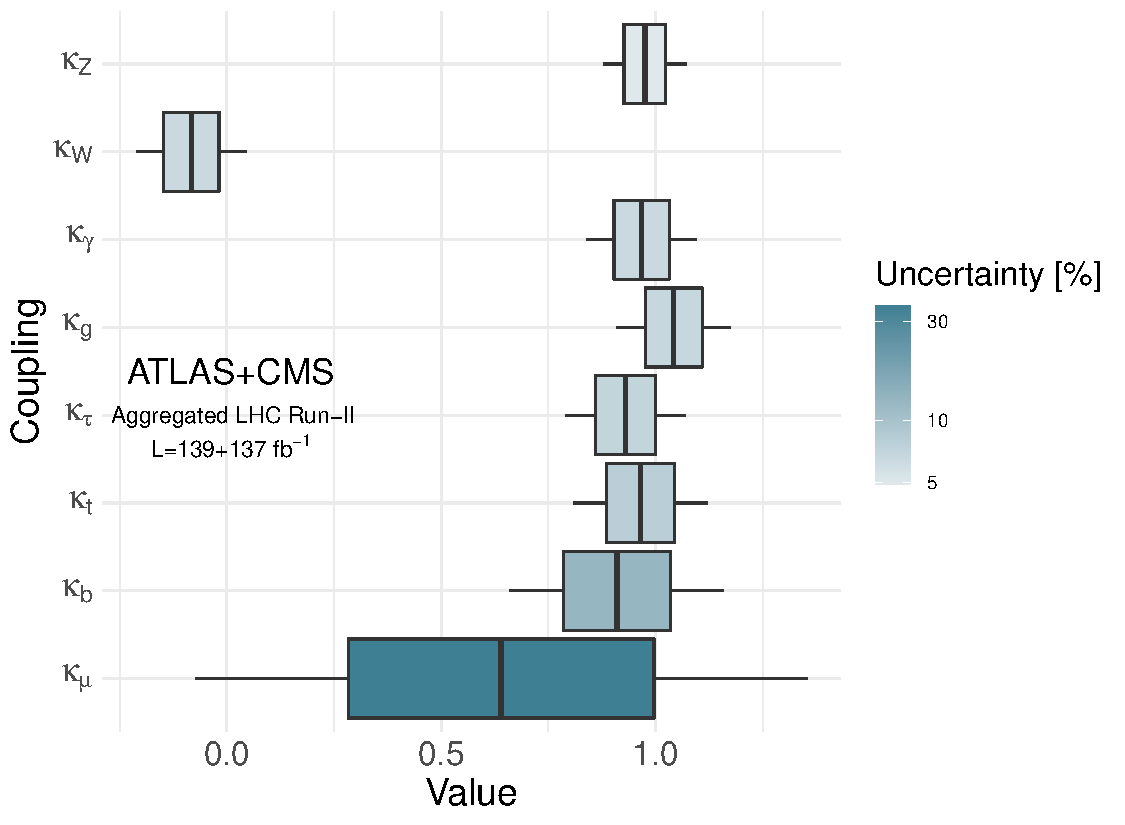
\includegraphics[height=0.3\textheight]{figures/agg_higgs_couplings}
		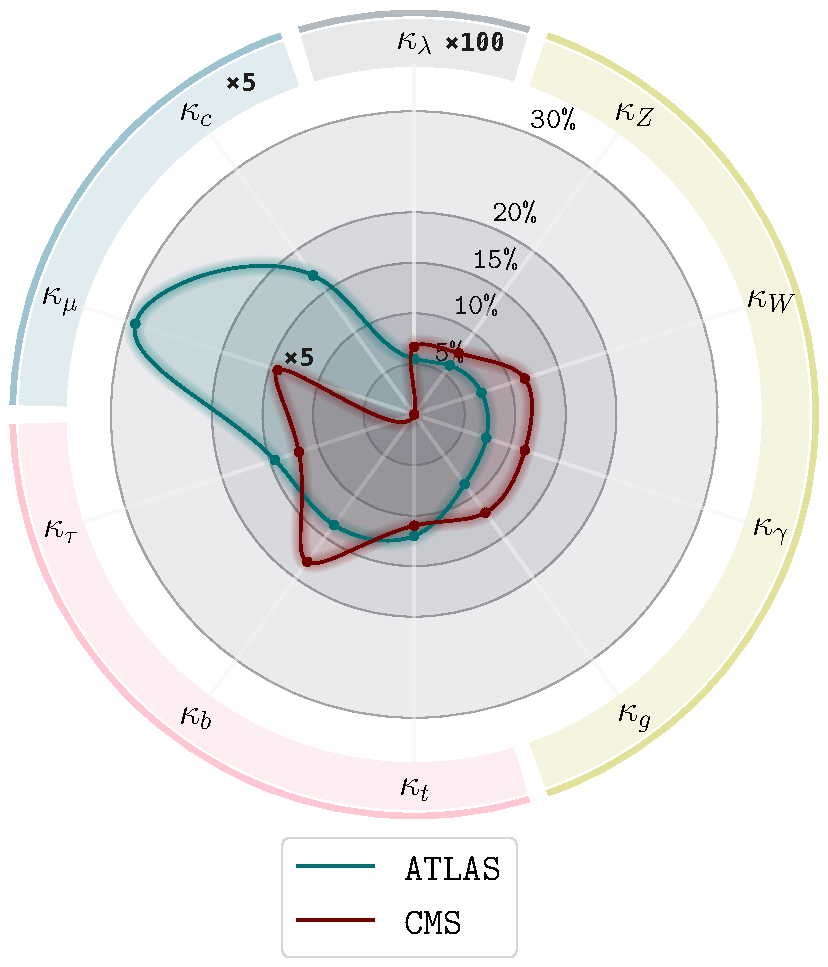
\includegraphics[height=0.3\textheight]{figures/Higgs_couplings_poster}
		\caption{(left) Meta-analysis aggregation of the most recent bounds from ATLAS~\cite{ATLAS2021vrm} and CMS~\cite{CMS:2020gsy} on the Higgs couplings modifiers $\kappa$. (right) The individual 68\% CI uncertainties on the coupling modifiers from ATLAS and CMS.   }	
		\label{fig:couplings-bound}
	\end{center}
\end{figure}
\par The measured bounds on the Higgs coupling to the gauge bosons, including the effective couplings to $\gamma$ and $g$, as well as the couplings to the third-generation fermions are within few percent of the SM prediction. The bounds on the coupling to the $W$ boson seems to favour a negative value in CMS fits, due to the channel used to constraint it $ h \to WW$  depending on $ \kappa_W^2$, thus making the best fit value of $ \sim -1$ within the SM prediction. An independent analysis on the relative signs of $\kappa_W$ and $\kappa_t$ was preformed using $th/t \bar{t} h$ processes in ref.~\cite{CMS:2018jeh}. Only the absolute value of $\kappa_W$ is reported in my combination of the analyses results.  Additionally,  the observation of the decays $ h \to b \bar{b}$~\cite{CMS:2018nsn,ATLAS:2018kot,ATLAS:2019yhn} and $h \to \tau \tau$~\cite{ATLAS:2018ynr,CMS:2019pyn} leads to direct measurements of the beauty and $\tau$ Yukawa couplings. This has made their bounds comparable to the gauge bosons and top couplings with the Higgs, with less than $10\%$ uncertainty. \textit{ Au contraire}, bounds on the Yukawa couplings of second and first generation fermions remain very weak.  
\par Recently, ATLAS  and CMS have preformed searches for the decay~$ h\to \mu \mu$~\cite{ATLAS:2020fzp,CMS:2020xwi} using the Run-II data. These searched have shown evidence o~($ 3 \sigma$) for  this decay. Consequently improving the constraints on $\kappa_\mu$, though as seen in ~\autoref{fig:couplings-bound}, the uncertainty remains high~$ \sim 36 \%$.  Studies on the Higgs decaying to charm pairs are significantly more challenging, and they have only permitted to set upper 95\% CL  bounds on $ |\kappa_c|$ of $8.5$ for ATLAS~\cite{ATLAS-CONF-2021-021,ATLAS:2022ers} and $70$ for CMS~\cite{CMS:2019hve}. There are no planned direct searches for the first generation Yukawa couplings (\emph{direct}) measurements planned for the LHC. It is not possible to directly access decays of the Higgs to up or down quarks at the LHC. Other methods for probing these couplings will be extensively discussed in ~\autoref{chap:lightyuk}.
\par By the end of the HL-LHC, it is projected that the couplings of the Higgs, including the ones with gauge bosons, third-generation fermions, and the muon Yukawa, will be measured at a few per cent level~\cite{Bernius:2666331}. This is highlighted by~\autoref{fig:couplings-hlhlc}, in this figure I show the improvement in the $\kappa$ measurement uncertainty expected by the HL-LHC compared to Run-II.
\begin{figure}[htb!]
	\begin{center}
		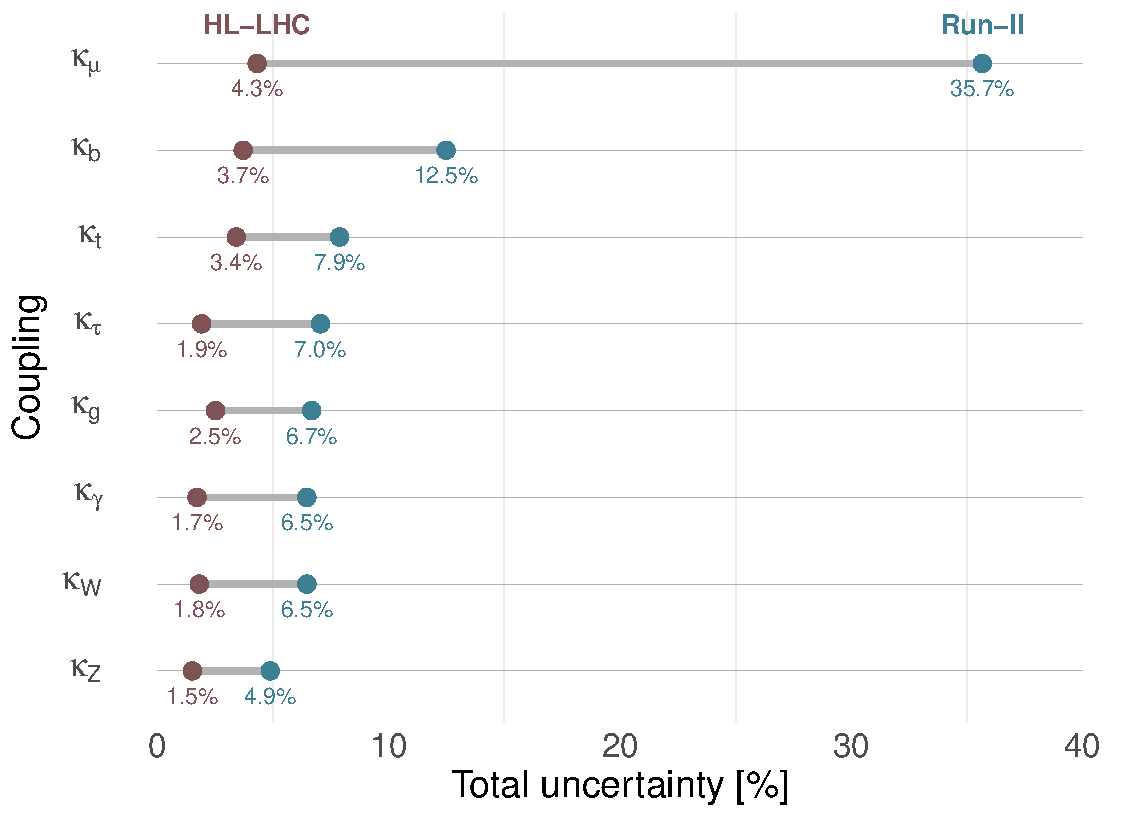
\includegraphics[height=0.35\textheight]{figures/run2-hl-dumble}
		\caption{Dumbbell plot illustrating the improvement of the uncertainties on the Higgs coupling's measurement projected for the HL-LHC compared to the current combined CMS and ATLAS measurements from Run-II data.}	
		\label{fig:couplings-hlhlc}
	\end{center}
\end{figure}
%\subsection{Miscellaneous Higgs measurements }
\section{Challenges and outlook \label{sec:Higgscouplchallenge} }
\par The future runs of the LHC  hold a lot of potential for further understanding  the properties of our 10-year old Higgs boson.  Although, for some processes and couplings there will still be a lot of challenges ahead. For instance, the observation of $h \to c \bar{c}$ will require highly efficient charm-tagging, which is expected to improve at the HL-LHC by a factor of 2.5~\cite{ATL-PHYS-PUB-2018-016}.  The signal strength of the rare decay~$ h \to Z \gamma$ currently is  only constrained to $3.6$ times the SM values at 95\% CL ~\cite{ATLAS:2020qcv} and it is expected to be measured at the HL-LHC with~$\sim 10\%$ uncertainty. 
\par Other Higgs boson couplings that we did not discuss above are the Higgs self-interactions (trilinear and quartic), as I have shown in~\autoref{pwusection} that the perturbative unitarity bound derived in ref.~\cite{DiLuzio:2017tfn} is the strongest on these couplings so far.  To experimentally measure Higgs self-couplings, it is imperative to observe multiple Higgs production. Namely, to access the trilinear self-coupling, Higgs pair production must be observed. Similarly, the quartic Higgs coupling measurement needs triple Higgs production observation. Woefully, these processes are experimentally arduous to detect, due to their low inclusive cross-section $\sim 30$ fb for~$hh$~\cite{Dawson:1998py} and $<0.1$ fb for $hhh$ at LHC maximum expected operational energy of $14$ TeV. The triple Higgs production will remain challenging even for future colliders, e.g. for the FCC-hh at $100$ TeV. This process has a cross-section of only $\sim 5$ fb~\cite{Papaefstathiou:2015paa}.  To put these numbers in the context of single Higgs production, recall the inclusive single-Higgs production cross-section of $\sim 70$ pb at the current LHC operation energy.  The triple Higgs production thus, will not be accessible at the LHC, and consequently, the quartic self-coupling will not be measured. However, the HL-LHC has a promising outlook to measure the trilinear self-coupling.
\par In ~\autoref{chap:4topSingleHiggs}, I will discuss the potential for using single-Higgs processes to indirectly probe the trilinear coupling, as proposed by several studies~\cite{McCullough:2013rea, Gorbahn:2016uoy, Degrassi:2016wml, Bizon:2016wgr, Maltoni:2017ims, Degrassi:2019yix, Degrassi:2021uik, Haisch:2021hvy} and the challenges accompanying it. Later in~\autoref{chap:overviewDiHiggs}, the Higgs pair production at the LHC will be overviewed along with the current and future searches for this process and the bounds from them on the trilinear Higgs self-coupling. 
\par Light quark Yukawa couplings are another example of formidable couplings to probe at the LHC. ~\autoref{chap:lightyuk} will be dedicated to overviewing the potential for Higgs pair production in the measurement of these elusive couplings. The focal point of that chapter will be multi-variate analysis in signal vs background separation.
